\PassOptionsToPackage{unicode=true}{hyperref} % options for packages loaded elsewhere
\PassOptionsToPackage{hyphens}{url}
%
\documentclass[]{book}
\usepackage{lmodern}
\usepackage{amssymb,amsmath}
\usepackage{ifxetex,ifluatex}
\usepackage{fixltx2e} % provides \textsubscript
\ifnum 0\ifxetex 1\fi\ifluatex 1\fi=0 % if pdftex
  \usepackage[T1]{fontenc}
  \usepackage[utf8]{inputenc}
  \usepackage{textcomp} % provides euro and other symbols
\else % if luatex or xelatex
  \usepackage{unicode-math}
  \defaultfontfeatures{Ligatures=TeX,Scale=MatchLowercase}
\fi
% use upquote if available, for straight quotes in verbatim environments
\IfFileExists{upquote.sty}{\usepackage{upquote}}{}
% use microtype if available
\IfFileExists{microtype.sty}{%
\usepackage[]{microtype}
\UseMicrotypeSet[protrusion]{basicmath} % disable protrusion for tt fonts
}{}
\IfFileExists{parskip.sty}{%
\usepackage{parskip}
}{% else
\setlength{\parindent}{0pt}
\setlength{\parskip}{6pt plus 2pt minus 1pt}
}
\usepackage{hyperref}
\hypersetup{
            pdftitle={Virgina Technical Report},
            pdfauthor={Shawn, Joe, D.A},
            pdfborder={0 0 0},
            breaklinks=true}
\urlstyle{same}  % don't use monospace font for urls
\usepackage{color}
\usepackage{fancyvrb}
\newcommand{\VerbBar}{|}
\newcommand{\VERB}{\Verb[commandchars=\\\{\}]}
\DefineVerbatimEnvironment{Highlighting}{Verbatim}{commandchars=\\\{\}}
% Add ',fontsize=\small' for more characters per line
\usepackage{framed}
\definecolor{shadecolor}{RGB}{248,248,248}
\newenvironment{Shaded}{\begin{snugshade}}{\end{snugshade}}
\newcommand{\AlertTok}[1]{\textcolor[rgb]{0.94,0.16,0.16}{#1}}
\newcommand{\AnnotationTok}[1]{\textcolor[rgb]{0.56,0.35,0.01}{\textbf{\textit{#1}}}}
\newcommand{\AttributeTok}[1]{\textcolor[rgb]{0.77,0.63,0.00}{#1}}
\newcommand{\BaseNTok}[1]{\textcolor[rgb]{0.00,0.00,0.81}{#1}}
\newcommand{\BuiltInTok}[1]{#1}
\newcommand{\CharTok}[1]{\textcolor[rgb]{0.31,0.60,0.02}{#1}}
\newcommand{\CommentTok}[1]{\textcolor[rgb]{0.56,0.35,0.01}{\textit{#1}}}
\newcommand{\CommentVarTok}[1]{\textcolor[rgb]{0.56,0.35,0.01}{\textbf{\textit{#1}}}}
\newcommand{\ConstantTok}[1]{\textcolor[rgb]{0.00,0.00,0.00}{#1}}
\newcommand{\ControlFlowTok}[1]{\textcolor[rgb]{0.13,0.29,0.53}{\textbf{#1}}}
\newcommand{\DataTypeTok}[1]{\textcolor[rgb]{0.13,0.29,0.53}{#1}}
\newcommand{\DecValTok}[1]{\textcolor[rgb]{0.00,0.00,0.81}{#1}}
\newcommand{\DocumentationTok}[1]{\textcolor[rgb]{0.56,0.35,0.01}{\textbf{\textit{#1}}}}
\newcommand{\ErrorTok}[1]{\textcolor[rgb]{0.64,0.00,0.00}{\textbf{#1}}}
\newcommand{\ExtensionTok}[1]{#1}
\newcommand{\FloatTok}[1]{\textcolor[rgb]{0.00,0.00,0.81}{#1}}
\newcommand{\FunctionTok}[1]{\textcolor[rgb]{0.00,0.00,0.00}{#1}}
\newcommand{\ImportTok}[1]{#1}
\newcommand{\InformationTok}[1]{\textcolor[rgb]{0.56,0.35,0.01}{\textbf{\textit{#1}}}}
\newcommand{\KeywordTok}[1]{\textcolor[rgb]{0.13,0.29,0.53}{\textbf{#1}}}
\newcommand{\NormalTok}[1]{#1}
\newcommand{\OperatorTok}[1]{\textcolor[rgb]{0.81,0.36,0.00}{\textbf{#1}}}
\newcommand{\OtherTok}[1]{\textcolor[rgb]{0.56,0.35,0.01}{#1}}
\newcommand{\PreprocessorTok}[1]{\textcolor[rgb]{0.56,0.35,0.01}{\textit{#1}}}
\newcommand{\RegionMarkerTok}[1]{#1}
\newcommand{\SpecialCharTok}[1]{\textcolor[rgb]{0.00,0.00,0.00}{#1}}
\newcommand{\SpecialStringTok}[1]{\textcolor[rgb]{0.31,0.60,0.02}{#1}}
\newcommand{\StringTok}[1]{\textcolor[rgb]{0.31,0.60,0.02}{#1}}
\newcommand{\VariableTok}[1]{\textcolor[rgb]{0.00,0.00,0.00}{#1}}
\newcommand{\VerbatimStringTok}[1]{\textcolor[rgb]{0.31,0.60,0.02}{#1}}
\newcommand{\WarningTok}[1]{\textcolor[rgb]{0.56,0.35,0.01}{\textbf{\textit{#1}}}}
\usepackage{longtable,booktabs}
% Fix footnotes in tables (requires footnote package)
\IfFileExists{footnote.sty}{\usepackage{footnote}\makesavenoteenv{longtable}}{}
\usepackage{graphicx,grffile}
\makeatletter
\def\maxwidth{\ifdim\Gin@nat@width>\linewidth\linewidth\else\Gin@nat@width\fi}
\def\maxheight{\ifdim\Gin@nat@height>\textheight\textheight\else\Gin@nat@height\fi}
\makeatother
% Scale images if necessary, so that they will not overflow the page
% margins by default, and it is still possible to overwrite the defaults
% using explicit options in \includegraphics[width, height, ...]{}
\setkeys{Gin}{width=\maxwidth,height=\maxheight,keepaspectratio}
\setlength{\emergencystretch}{3em}  % prevent overfull lines
\providecommand{\tightlist}{%
  \setlength{\itemsep}{0pt}\setlength{\parskip}{0pt}}
\setcounter{secnumdepth}{5}
% Redefines (sub)paragraphs to behave more like sections
\ifx\paragraph\undefined\else
\let\oldparagraph\paragraph
\renewcommand{\paragraph}[1]{\oldparagraph{#1}\mbox{}}
\fi
\ifx\subparagraph\undefined\else
\let\oldsubparagraph\subparagraph
\renewcommand{\subparagraph}[1]{\oldsubparagraph{#1}\mbox{}}
\fi

% set default figure placement to htbp
\makeatletter
\def\fps@figure{htbp}
\makeatother

\usepackage{booktabs}
\usepackage{amsthm}
\makeatletter
\def\thm@space@setup{%
  \thm@preskip=8pt plus 2pt minus 4pt
  \thm@postskip=\thm@preskip
}
\makeatother
\usepackage[]{natbib}
\bibliographystyle{apalike}

\title{Virgina Technical Report}
\author{Shawn, Joe, D.A}
\date{2020-11-18}

\begin{document}
\maketitle

{
\setcounter{tocdepth}{1}
\tableofcontents
}
\hypertarget{prerequisites}{%
\chapter{Prerequisites}\label{prerequisites}}

This is a \emph{sample} book written in \textbf{Markdown}. You can use anything that Pandoc's Markdown supports, e.g., a math equation \(a^2 + b^2 = c^2\).

The \textbf{bookdown} package can be installed from CRAN or Github:

\begin{Shaded}
\begin{Highlighting}[]
\KeywordTok{install.packages}\NormalTok{(}\StringTok{"bookdown"}\NormalTok{)}
\CommentTok{# or the development version}
\CommentTok{# devtools::install_github("rstudio/bookdown")}
\end{Highlighting}
\end{Shaded}

Remember each Rmd file contains one and only one chapter, and a chapter is defined by the first-level heading \texttt{\#}.

To compile this example to PDF, you need XeLaTeX. You are recommended to install TinyTeX (which includes XeLaTeX): \url{https://yihui.name/tinytex/}.

\hypertarget{intro}{%
\chapter{Introduction}\label{intro}}

It is the policy of the State Board of Education and a priority of the Virgina
Department of Education that there will be no discrimination or harassment on
the grounds of race, color, religion, sex, sexual orientation, national origin,
age or disability in any educational programs, activities or employment. Persons
having questions about equal opportunity and nondiscrimination should contact
the Deputy Superintendent of Public Instruction with the Virgina Department of
Education.
*This technical report is one of a series that describes the development of
Virgina's Statewide Assessment System. The complete set of volumes provides
comprehensive documentation of the development, procedures, technical adequacy,
and results of the system.

\newpage

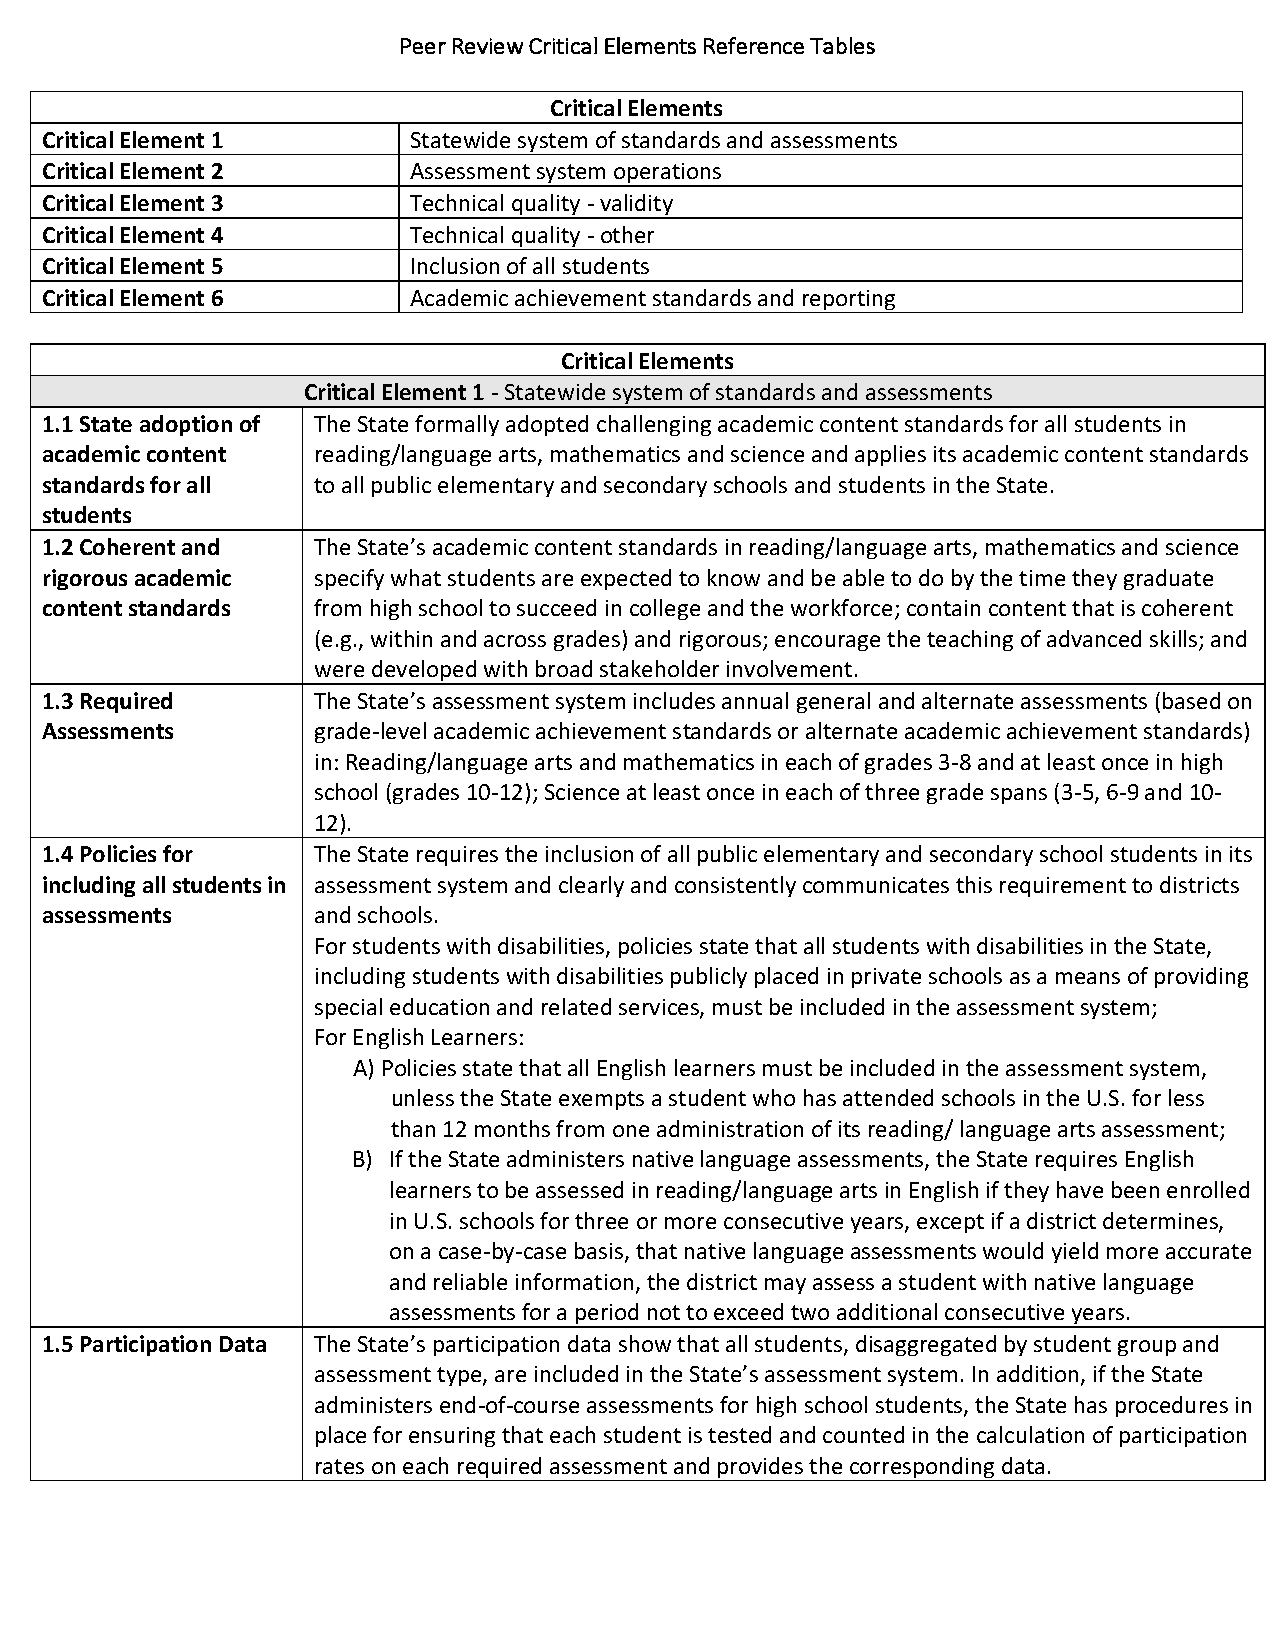
\includegraphics{figures/peer_rev/Critical_Elements_Reference_Tables.pdf}

\newpage

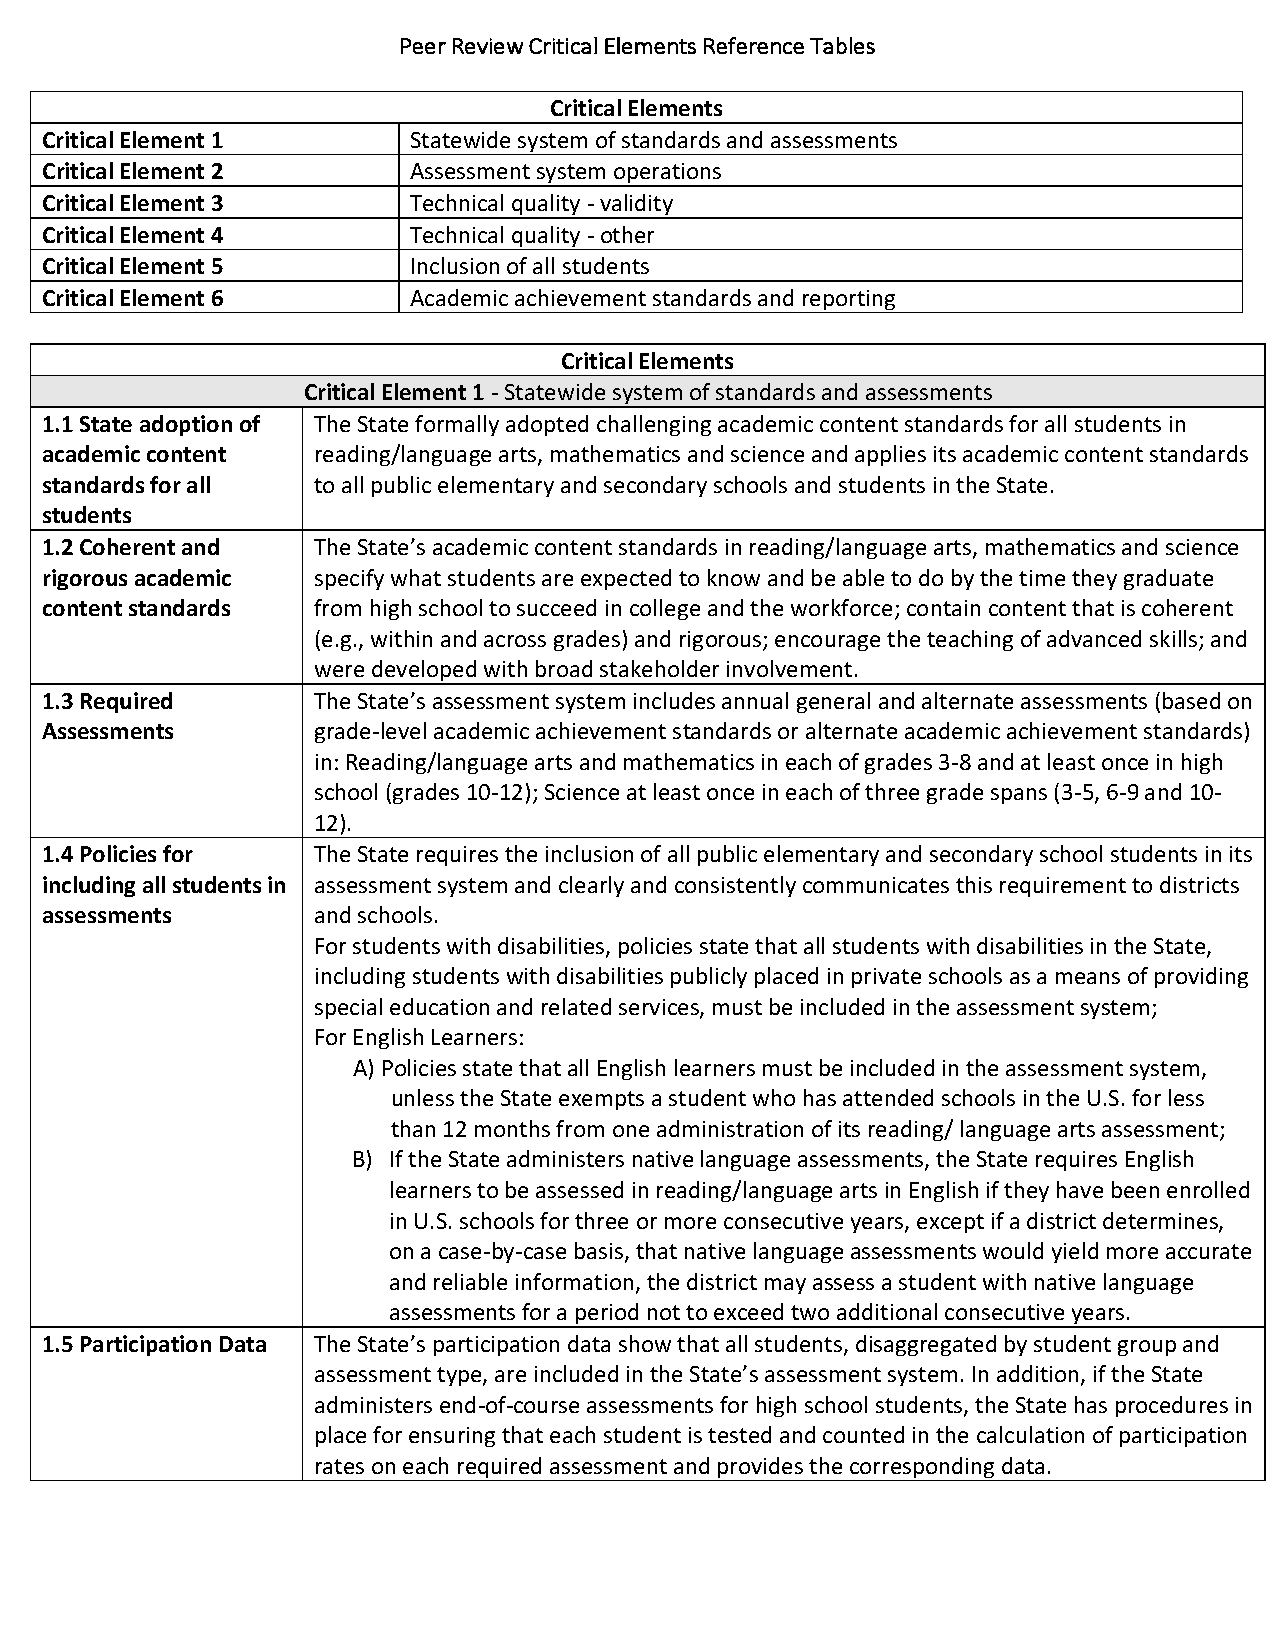
\includegraphics{figures/peer_rev/PeerReview1.pdf}

\newpage

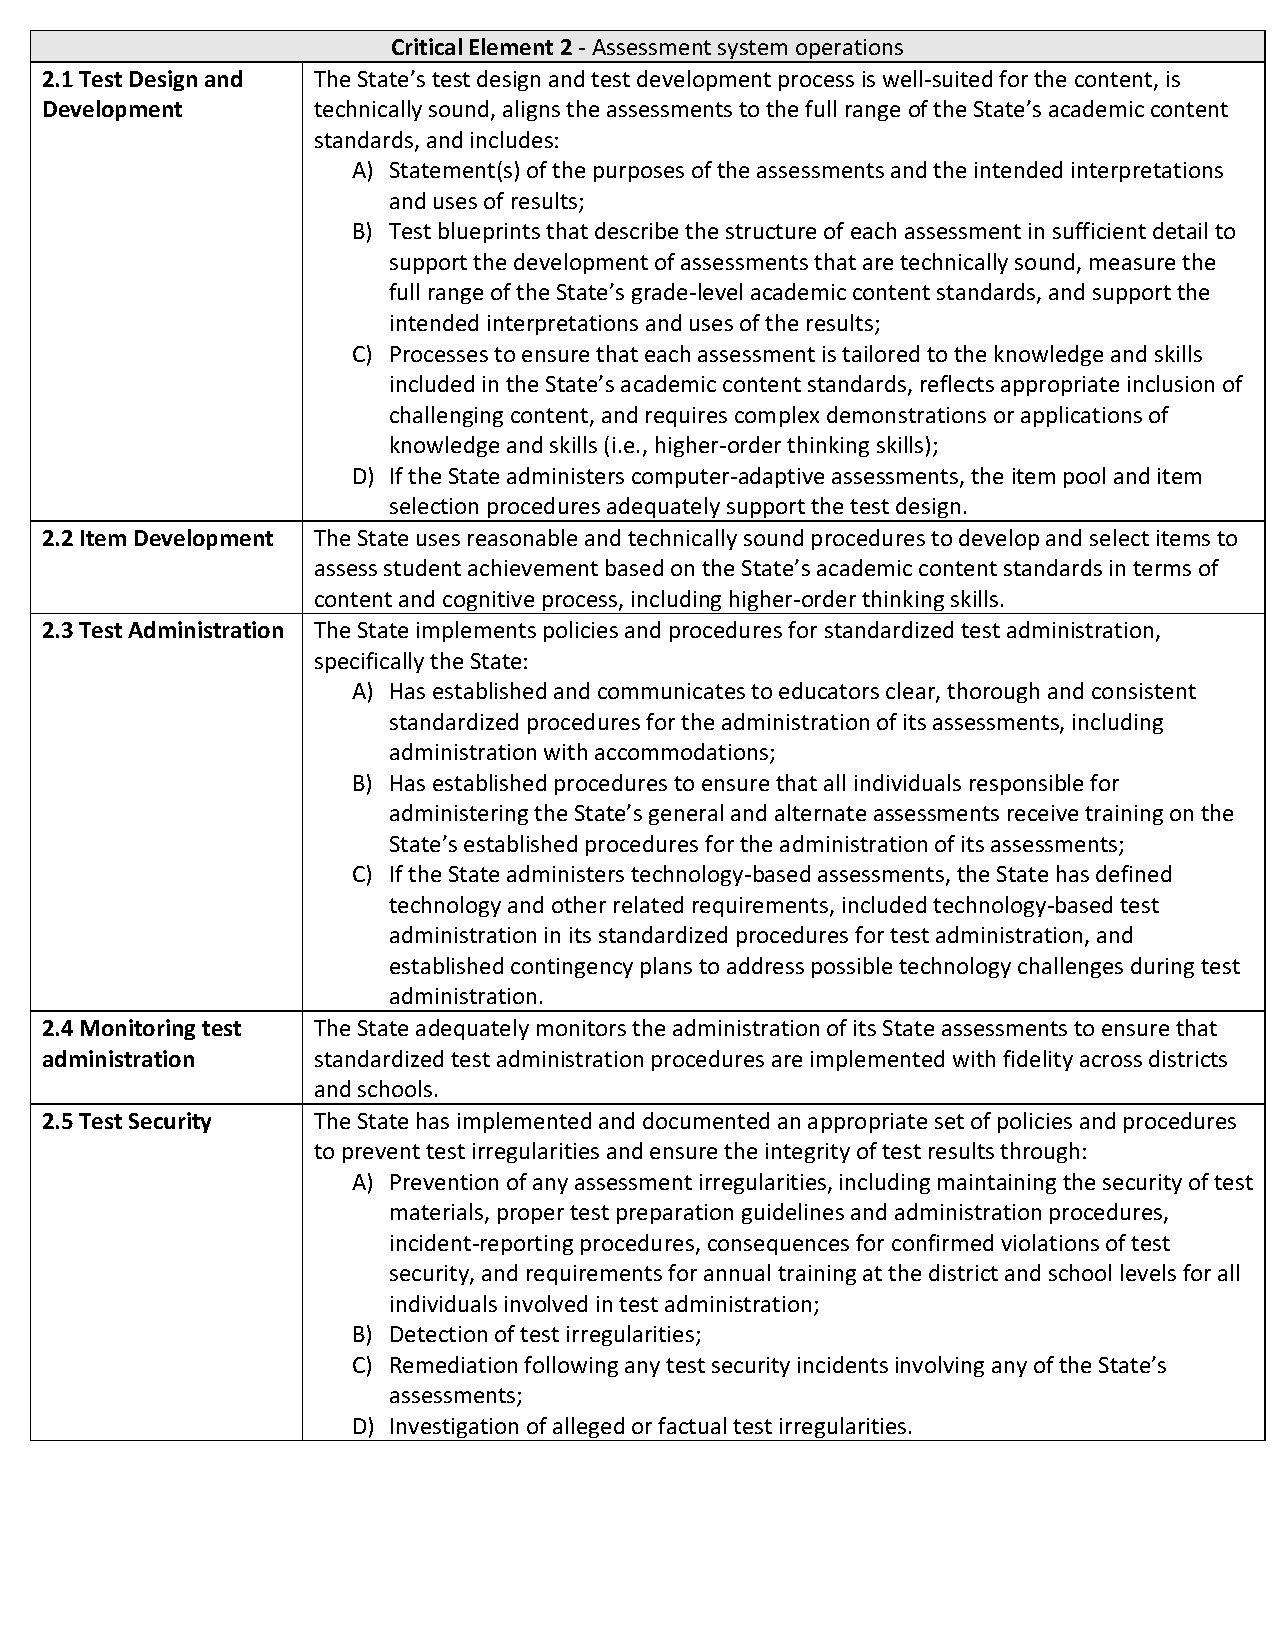
\includegraphics{figures/peer_rev/PeerReview2.pdf}

\newpage

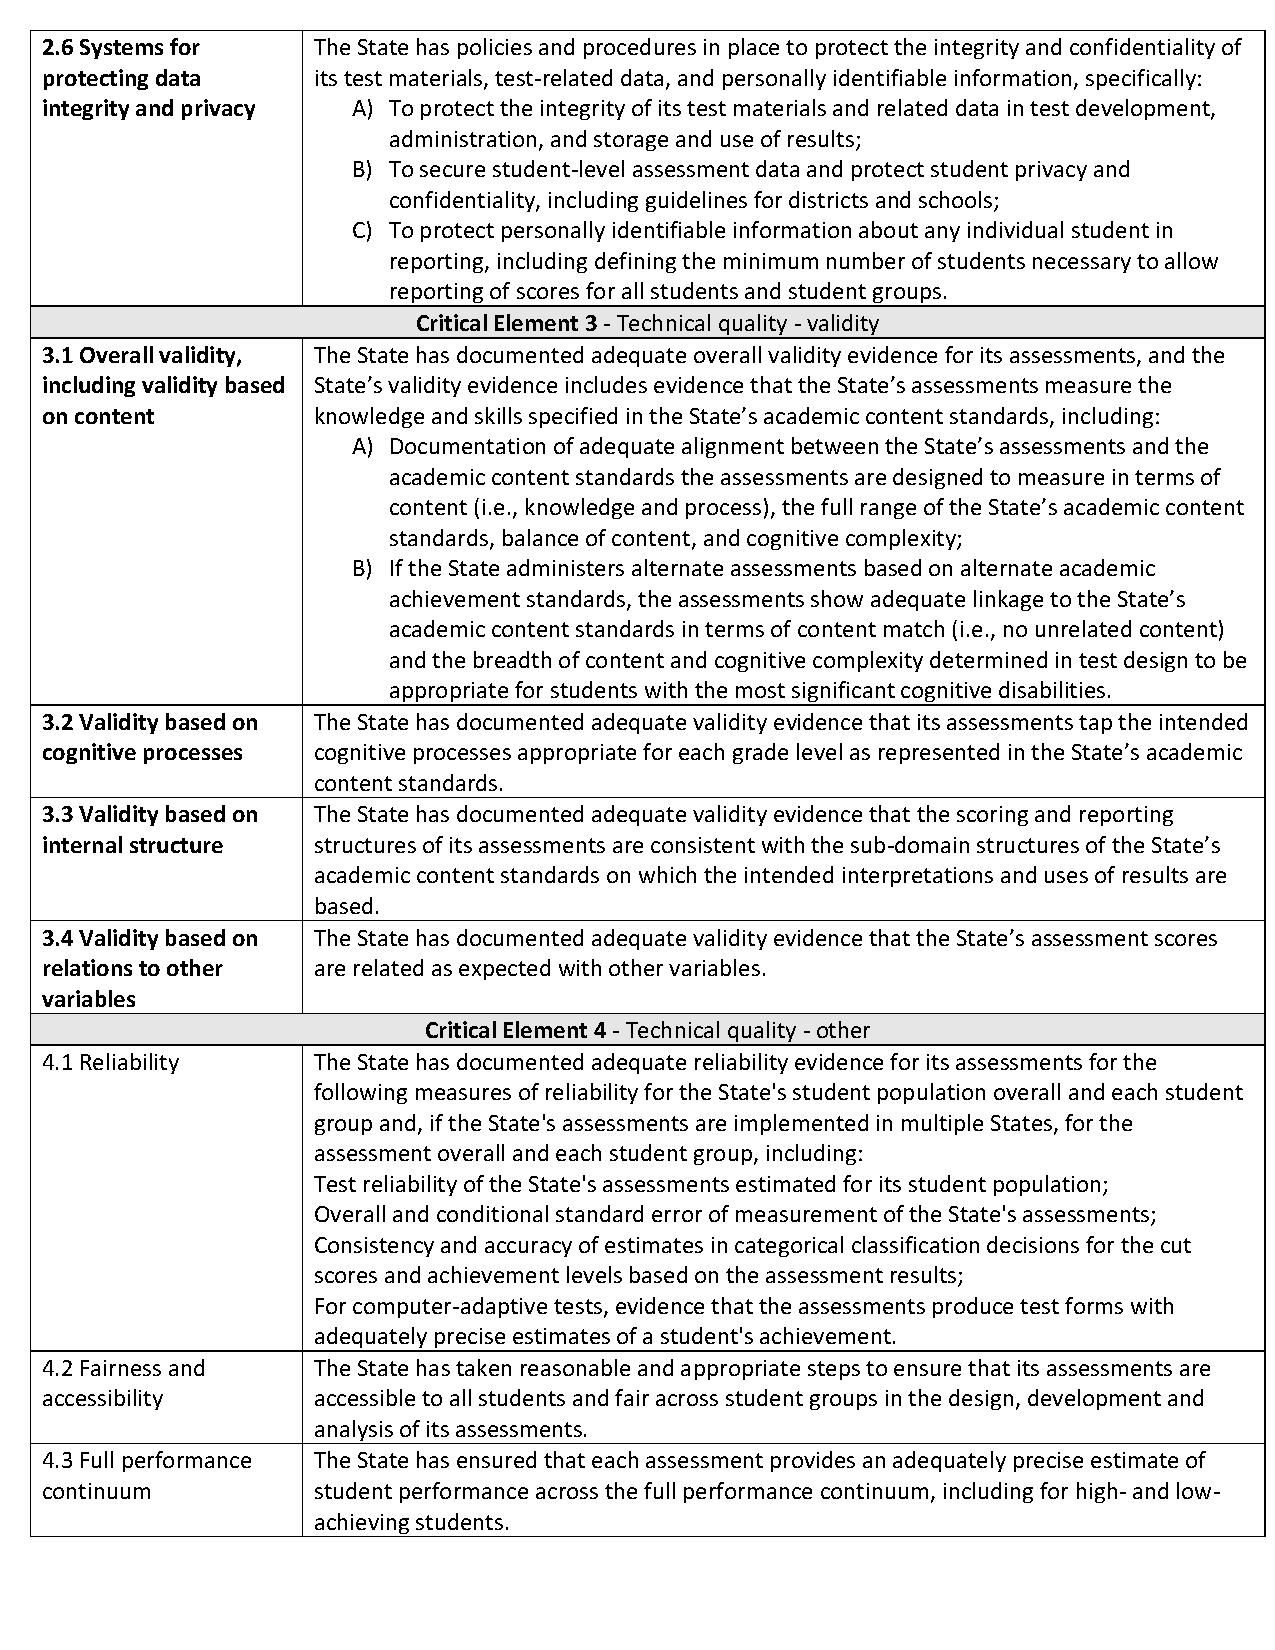
\includegraphics{figures/peer_rev/PeerReview3.pdf}

\newpage

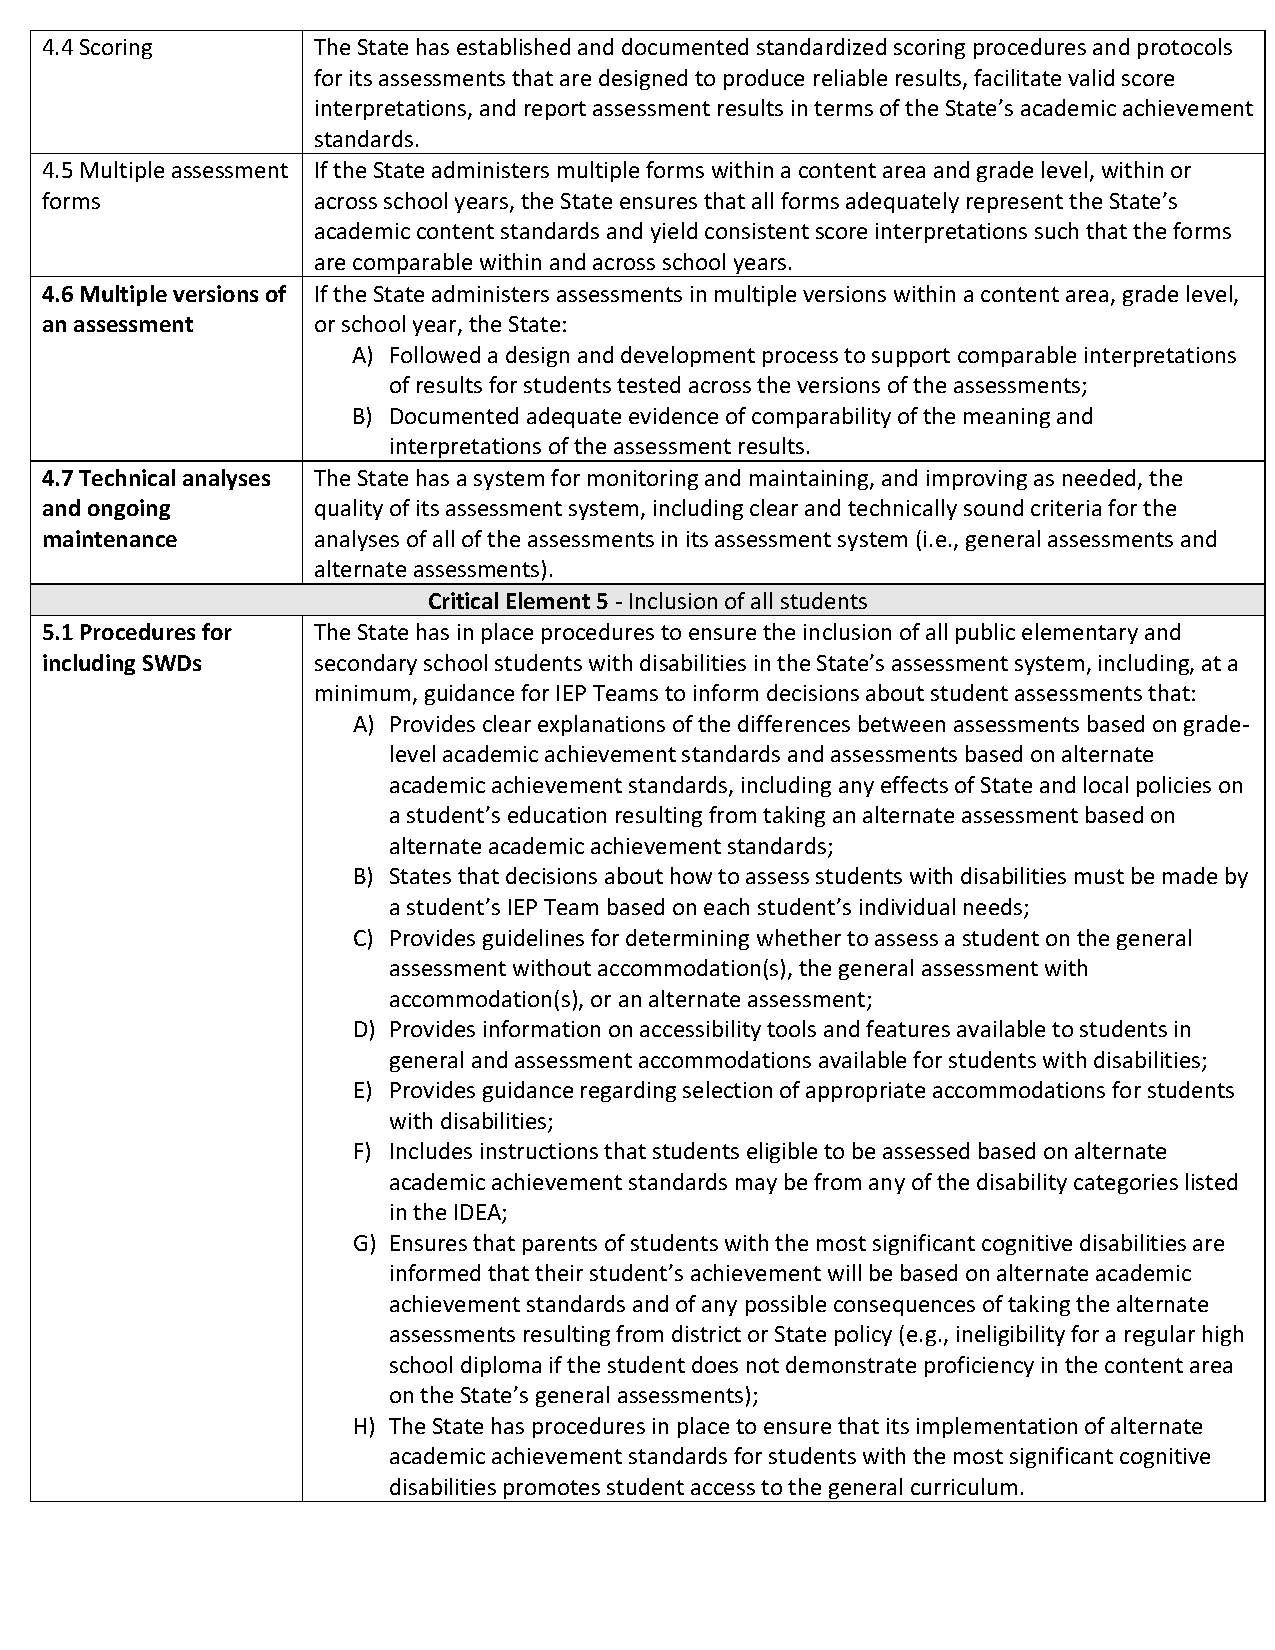
\includegraphics{figures/peer_rev/PeerReview4.pdf}

\newpage

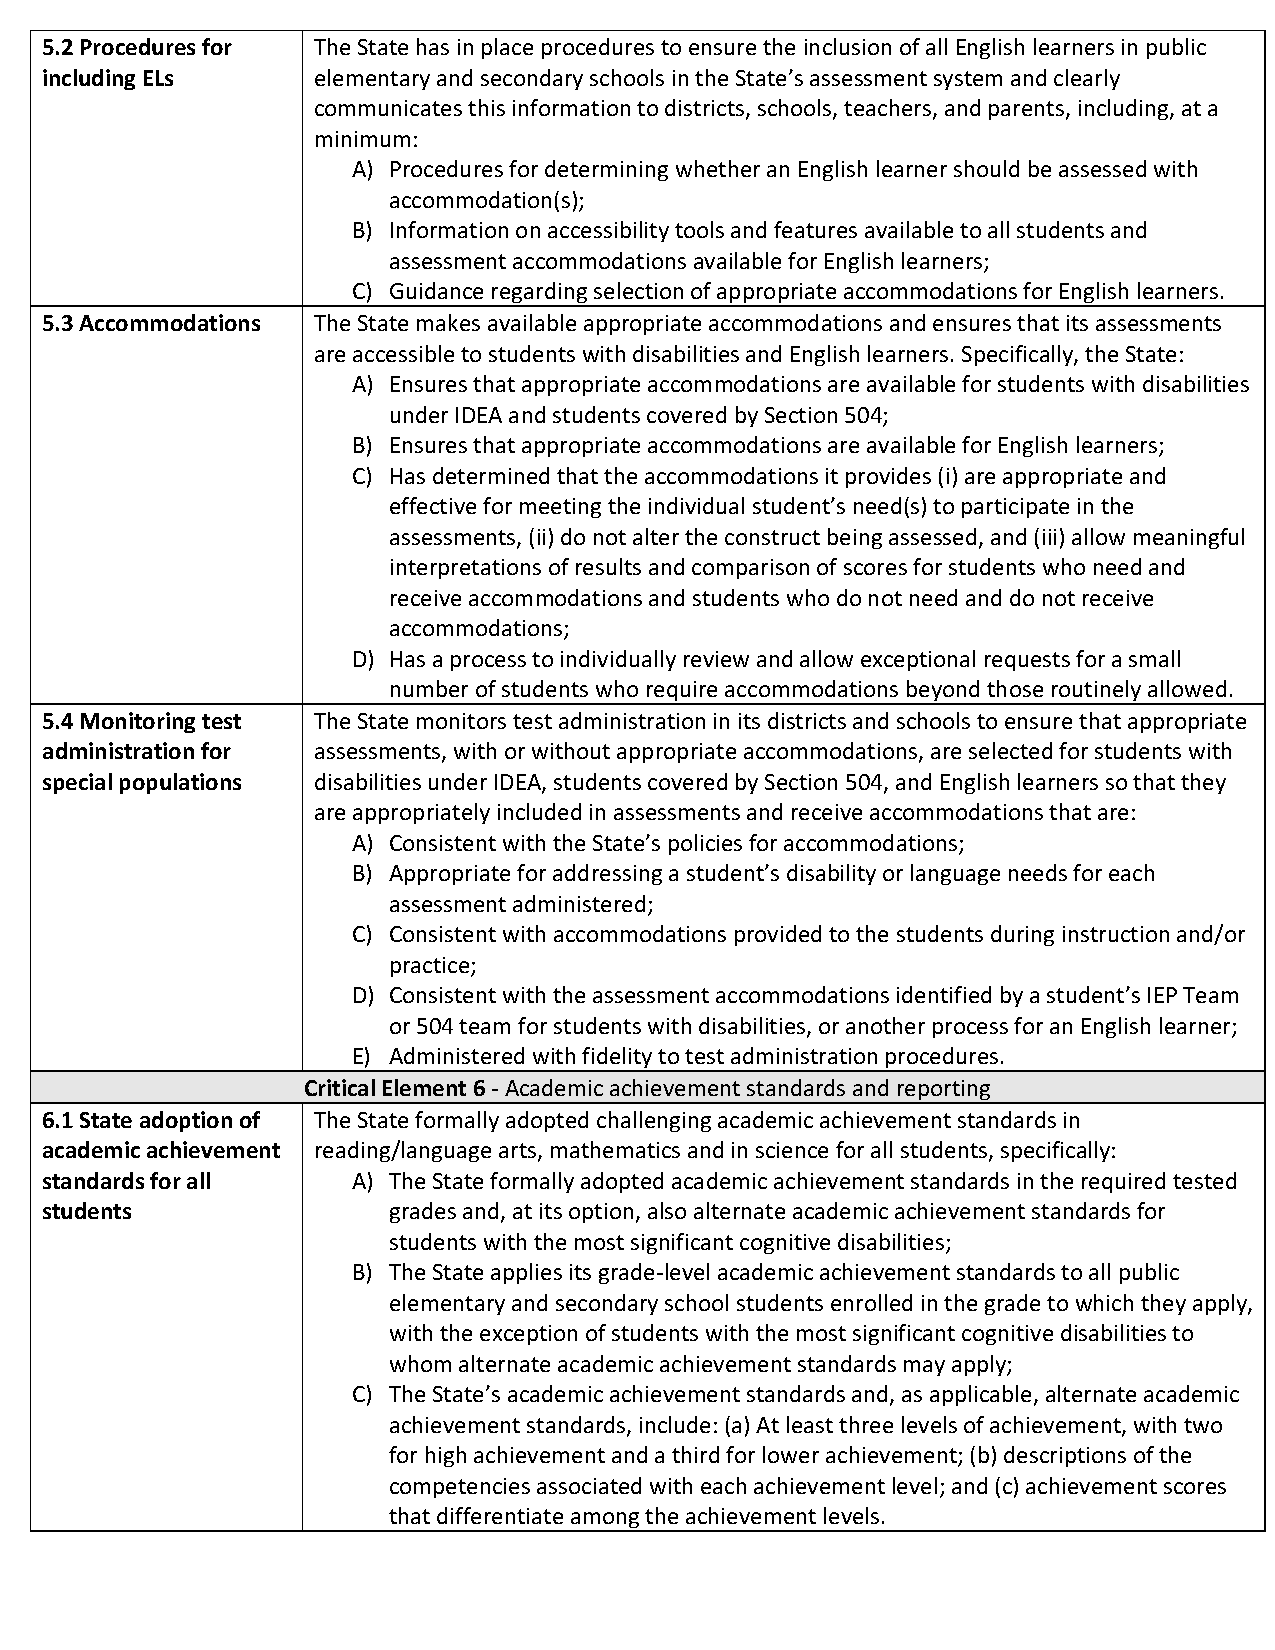
\includegraphics{figures/peer_rev/PeerReview5.pdf}

\newpage

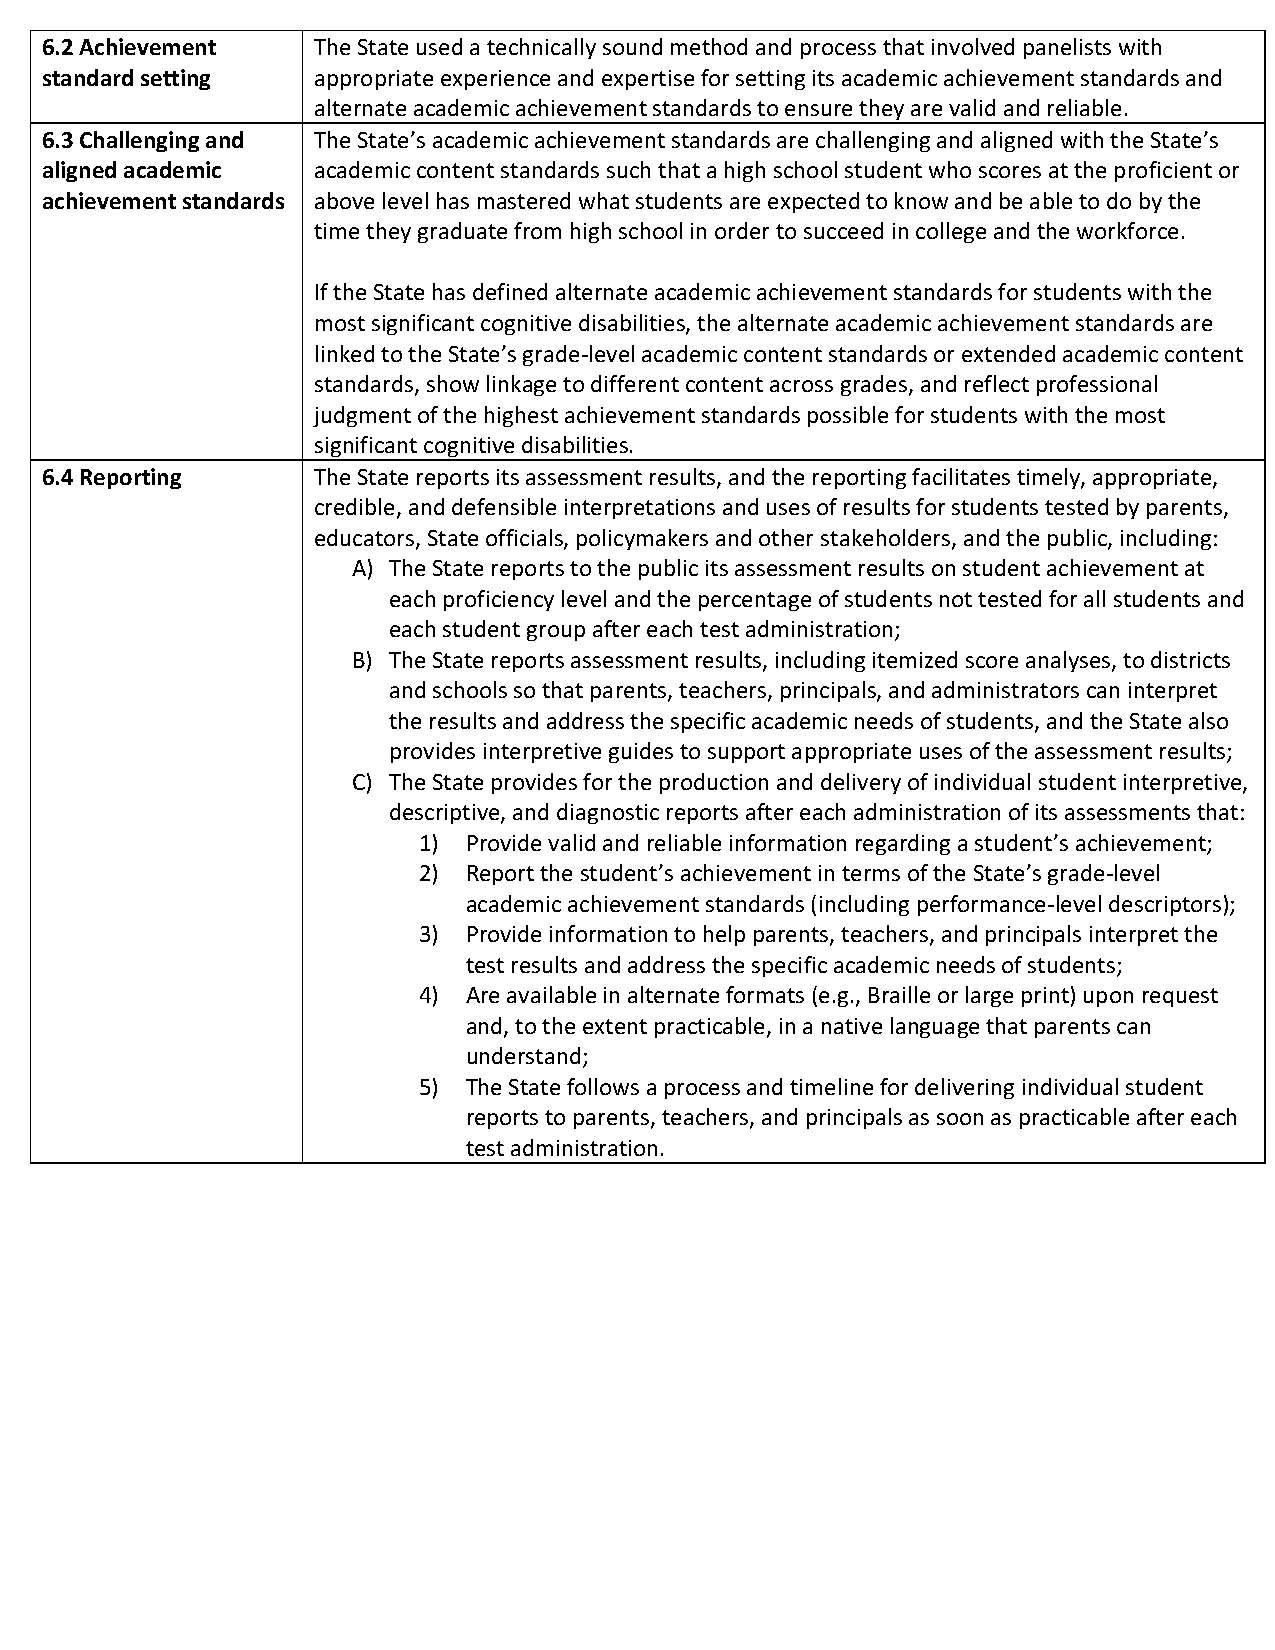
\includegraphics{figures/peer_rev/PeerReview6.pdf}

You can label chapter and section titles using \texttt{\{\#label\}} after them, e.g., we can reference Chapter \ref{intro}. If you do not manually label them, there will be automatic labels anyway, e.g., Chapter \ref{methods}.

\begin{Shaded}
\begin{Highlighting}[]
\CommentTok{#bookdown::render_book("index.Rmd")}
\end{Highlighting}
\end{Shaded}

Figures and tables with captions will be placed in \texttt{figure} and \texttt{table} environments, respectively.

\begin{Shaded}
\begin{Highlighting}[]
\KeywordTok{par}\NormalTok{(}\DataTypeTok{mar =} \KeywordTok{c}\NormalTok{(}\DecValTok{4}\NormalTok{, }\DecValTok{4}\NormalTok{, }\FloatTok{.1}\NormalTok{, }\FloatTok{.1}\NormalTok{))}
\KeywordTok{plot}\NormalTok{(pressure, }\DataTypeTok{type =} \StringTok{'b'}\NormalTok{, }\DataTypeTok{pch =} \DecValTok{19}\NormalTok{)}
\end{Highlighting}
\end{Shaded}

\begin{figure}

{\centering 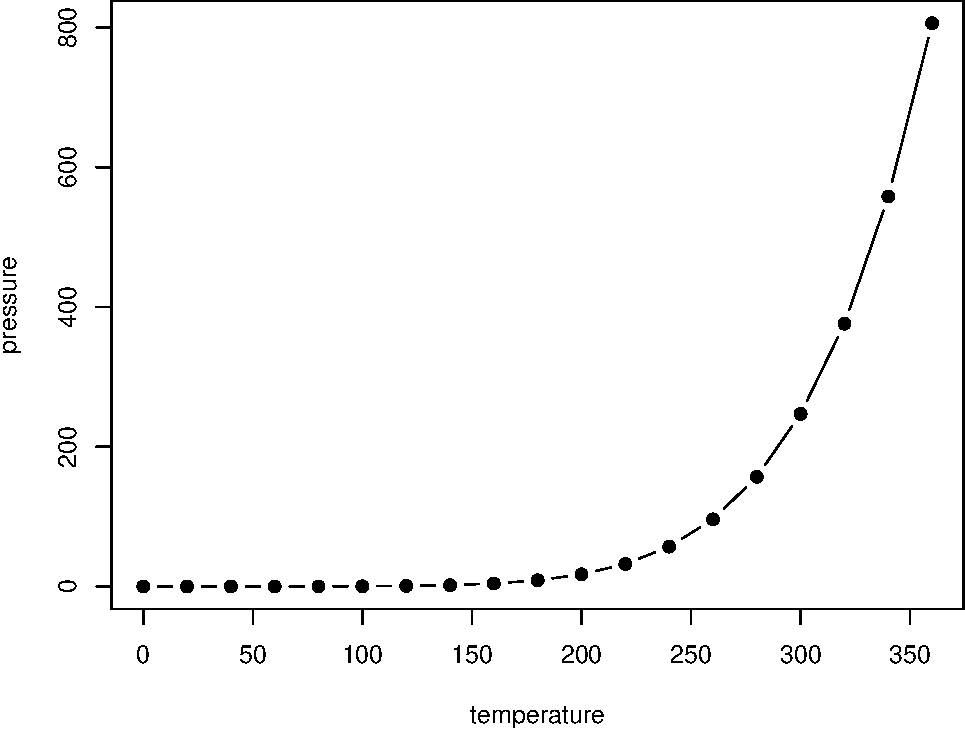
\includegraphics[width=0.8\linewidth]{bookdown-demo_files/figure-latex/nice-fig-1} 

}

\caption{Here is a nice figure!}\label{fig:nice-fig}
\end{figure}

Reference a figure by its code chunk label with the \texttt{fig:} prefix, e.g., see Figure \ref{fig:nice-fig}. Similarly, you can reference tables generated from \texttt{knitr::kable()}, e.g., see Table \ref{tab:nice-tab}.

\begin{Shaded}
\begin{Highlighting}[]
\NormalTok{knitr}\OperatorTok{::}\KeywordTok{kable}\NormalTok{(}
  \KeywordTok{head}\NormalTok{(iris, }\DecValTok{20}\NormalTok{), }\DataTypeTok{caption =} \StringTok{'Here is a nice table!'}\NormalTok{,}
  \DataTypeTok{booktabs =} \OtherTok{TRUE}
\NormalTok{)}
\end{Highlighting}
\end{Shaded}

\begin{table}

\caption{\label{tab:nice-tab}Here is a nice table!}
\centering
\begin{tabular}[t]{rrrrl}
\toprule
Sepal.Length & Sepal.Width & Petal.Length & Petal.Width & Species\\
\midrule
5.1 & 3.5 & 1.4 & 0.2 & setosa\\
4.9 & 3.0 & 1.4 & 0.2 & setosa\\
4.7 & 3.2 & 1.3 & 0.2 & setosa\\
4.6 & 3.1 & 1.5 & 0.2 & setosa\\
5.0 & 3.6 & 1.4 & 0.2 & setosa\\
\addlinespace
5.4 & 3.9 & 1.7 & 0.4 & setosa\\
4.6 & 3.4 & 1.4 & 0.3 & setosa\\
5.0 & 3.4 & 1.5 & 0.2 & setosa\\
4.4 & 2.9 & 1.4 & 0.2 & setosa\\
4.9 & 3.1 & 1.5 & 0.1 & setosa\\
\addlinespace
5.4 & 3.7 & 1.5 & 0.2 & setosa\\
4.8 & 3.4 & 1.6 & 0.2 & setosa\\
4.8 & 3.0 & 1.4 & 0.1 & setosa\\
4.3 & 3.0 & 1.1 & 0.1 & setosa\\
5.8 & 4.0 & 1.2 & 0.2 & setosa\\
\addlinespace
5.7 & 4.4 & 1.5 & 0.4 & setosa\\
5.4 & 3.9 & 1.3 & 0.4 & setosa\\
5.1 & 3.5 & 1.4 & 0.3 & setosa\\
5.7 & 3.8 & 1.7 & 0.3 & setosa\\
5.1 & 3.8 & 1.5 & 0.3 & setosa\\
\bottomrule
\end{tabular}
\end{table}

You can write citations, too. For example, we are using the \textbf{bookdown} package \citep{R-bookdown} in this sample book, which was built on top of R Markdown and \textbf{knitr} \citep{xie2015}.

\hypertarget{critical-element-1-statewide-system-of-standards-and-assessments}{%
\chapter{Critical Element 1 Statewide system of standards and assessments}\label{critical-element-1-statewide-system-of-standards-and-assessments}}

\hypertarget{state-adoption-of-academic-content-standards-for-all-students}{%
\subsection{1.1 State Adoption of Academic Content Standards for All Students}\label{state-adoption-of-academic-content-standards-for-all-students}}

\hypertarget{coherent-and-rigorous-academic-content-standards}{%
\subsection{1.2 Coherent and Rigorous Academic Content Standards}\label{coherent-and-rigorous-academic-content-standards}}

\hypertarget{required-assessments}{%
\subsection{1.3 Required Assessments}\label{required-assessments}}

\hypertarget{policies-for-including-all-students-in-assessments}{%
\subsection{1.4 Policies for Including All Students in Assessments}\label{policies-for-including-all-students-in-assessments}}

\hypertarget{a-english-learners}{%
\subsubsection{1.4A English Learners}\label{a-english-learners}}

\hypertarget{b-native-language-assessments}{%
\subsubsection{1.4B Native Language Assessments}\label{b-native-language-assessments}}

\hypertarget{participation-data}{%
\subsection{1.5 Participation Data}\label{participation-data}}

\hypertarget{critical-element-2-assessment-system-operations}{%
\chapter{Critical Element 2 Assessment system operations}\label{critical-element-2-assessment-system-operations}}

\hypertarget{test-design-and-development}{%
\subsection{2.1 Test Design and Development}\label{test-design-and-development}}

\hypertarget{a-vaext-purpose}{%
\subsubsection{2.1A VAExt Purpose}\label{a-vaext-purpose}}

\hypertarget{b-vaext-test-blueprint}{%
\subsubsection{2.1B VAExt Test Blueprint}\label{b-vaext-test-blueprint}}

\hypertarget{c-test-development-processes}{%
\subsubsection{2.1C Test Development Processes}\label{c-test-development-processes}}

\hypertarget{d-computer-adaptive-considerations}{%
\subsubsection{2.1D Computer-Adaptive Considerations}\label{d-computer-adaptive-considerations}}

\hypertarget{item-development}{%
\subsection{2.2 Item Development}\label{item-development}}

\hypertarget{critical-element-3-technical-quality---validity}{%
\chapter{Critical Element 3 Technical Quality - Validity}\label{critical-element-3-technical-quality---validity}}

\hypertarget{overall-validity-including-validity-based-on-content}{%
\subsection{3.1 Overall Validity, Including Validity Based on Content}\label{overall-validity-including-validity-based-on-content}}

\hypertarget{a-alignment-between-aa-aaas-and-academic-content-standards}{%
\subsubsection{3.1A Alignment Between AA-AAAS and Academic Content Standards}\label{a-alignment-between-aa-aaas-and-academic-content-standards}}

\hypertarget{b-aa-aaas-linkage-to-general-content-standards}{%
\subsubsection{3.1B AA-AAAS Linkage to General Content Standards}\label{b-aa-aaas-linkage-to-general-content-standards}}

\hypertarget{validity-based-on-cognitive-processes}{%
\subsection{3.2 Validity Based on Cognitive Processes}\label{validity-based-on-cognitive-processes}}

\hypertarget{validity-based-on-internal-structure-content-and-function}{%
\subsection{3.3 Validity Based on Internal Structure (Content and Function)}\label{validity-based-on-internal-structure-content-and-function}}

\hypertarget{critical-element-4-technical-quality---other}{%
\chapter{Critical Element 4 Technical Quality - other}\label{critical-element-4-technical-quality---other}}

\hypertarget{reliability}{%
\subsection{4.1 Reliability}\label{reliability}}

\hypertarget{inter-rater-reliability}{%
\subsubsection{Inter-Rater-Reliability}\label{inter-rater-reliability}}

\hypertarget{background}{%
\paragraph{Background}\label{background}}

\hypertarget{methods}{%
\paragraph{Methods}\label{methods}}

\hypertarget{domain-definitions}{%
\subparagraph{Domain Definitions}\label{domain-definitions}}

\hypertarget{critical-element-5-inclusion-of-all-students}{%
\chapter{Critical Element 5 Inclusion of all students}\label{critical-element-5-inclusion-of-all-students}}

\hypertarget{procedures-for-including-swds}{%
\subsection{5.1 Procedures for Including SWDs}\label{procedures-for-including-swds}}

\hypertarget{a-clear-explanations-of-the-differences-between-assessments}{%
\subsubsection{5.1A Clear Explanations of the Differences Between Assessments}\label{a-clear-explanations-of-the-differences-between-assessments}}

\hypertarget{b-eligibility-decisions-made-by-iep-teams}{%
\subsubsection{5.1B Eligibility Decisions Made by IEP Teams}\label{b-eligibility-decisions-made-by-iep-teams}}

\hypertarget{c-guidelines-for-assessment-selection}{%
\subsubsection{5.1C Guidelines for Assessment Selection}\label{c-guidelines-for-assessment-selection}}

\hypertarget{d-information-on-accessibility-options}{%
\subsubsection{5.1D Information on Accessibility Options}\label{d-information-on-accessibility-options}}

\hypertarget{e-guidance-regarding-appropriate-accommodations}{%
\subsubsection{5.1E Guidance Regarding Appropriate Accommodations}\label{e-guidance-regarding-appropriate-accommodations}}

\hypertarget{f-all-swds-eligible-for-the-vaext}{%
\subsubsection{5.1F All SWDs Eligible for the VAExt}\label{f-all-swds-eligible-for-the-vaext}}

\hypertarget{g-parents-informed-of-aa-aaas-consequences}{%
\subsubsection{5.1G Parents Informed of AA-AAAS Consequences}\label{g-parents-informed-of-aa-aaas-consequences}}

\hypertarget{h-state-ensures-vaext-promotes-access-to-the-general-education-curriculum}{%
\subsubsection{5.1H State Ensures VAExt Promotes Access to the General Education Curriculum}\label{h-state-ensures-vaext-promotes-access-to-the-general-education-curriculum}}

\hypertarget{a---5.2c-procedures-for-including-els}{%
\subsection{5.2A - 5.2C Procedures for Including ELs}\label{a---5.2c-procedures-for-including-els}}

\hypertarget{accommodations}{%
\subsection{5.3 Accommodations}\label{accommodations}}

\hypertarget{a-appropriate-accommodations-are-available-for-swd-section-504}{%
\subsubsection{5.3A Appropriate Accommodations are Available for SWD/ Section 504}\label{a-appropriate-accommodations-are-available-for-swd-section-504}}

\hypertarget{b-appropriate-accommodations-are-available-for-els}{%
\subsubsection{5.3B Appropriate Accommodations are Available for ELs}\label{b-appropriate-accommodations-are-available-for-els}}

\hypertarget{c-accommodations-are-appropriate-and-effective}{%
\subsubsection{5.3C Accommodations are Appropriate and Effective}\label{c-accommodations-are-appropriate-and-effective}}

\hypertarget{d-accommodations-are-appropriate-and-effective}{%
\subsubsection{5.3D Accommodations are Appropriate and Effective}\label{d-accommodations-are-appropriate-and-effective}}

\hypertarget{a---5.4e-monitoring-test-administration-for-special-populations}{%
\subsection{5.4A - 5.4E Monitoring Test Administration for Special Populations}\label{a---5.4e-monitoring-test-administration-for-special-populations}}

\hypertarget{critical-element-6-academic-achievement-standards-and-reporting}{%
\chapter{Critical Element 6 Academic achievement standards and reporting}\label{critical-element-6-academic-achievement-standards-and-reporting}}

\hypertarget{state-adoption-of-alternate-academic-achievement-standards-for-swscd}{%
\subsection{6.1 State Adoption of Alternate Academic Achievement Standards for SWSCD}\label{state-adoption-of-alternate-academic-achievement-standards-for-swscd}}

\hypertarget{a-state-formally-adopted-alternate-academic-achievement-standards}{%
\subsubsection{6.1A State Formally Adopted Alternate Academic Achievement Standards}\label{a-state-formally-adopted-alternate-academic-achievement-standards}}

\hypertarget{b-state-applies-aaas-to-all-public-school-swscd-in-tested-grades}{%
\subsubsection{6.1B State Applies AAAS to All Public School SWSCD in Tested Grades}\label{b-state-applies-aaas-to-all-public-school-swscd-in-tested-grades}}

\hypertarget{c-states-aaas-include-at-least-three-levels-alds-and-cut-scores}{%
\subsubsection{6.1C State's AAAS Include At Least Three Levels, ALDs, and Cut Scores}\label{c-states-aaas-include-at-least-three-levels-alds-and-cut-scores}}

\hypertarget{achievement-standard-setting}{%
\subsection{6.2 Achievement Standard Setting}\label{achievement-standard-setting}}

\bibliography{book.bib,packages.bib}

\end{document}
